\documentclass[tikz,border=8pt]{standalone}
% Shared look for every TikZ diagram. Load with % Shared look for every TikZ diagram. Load with % Shared look for every TikZ diagram. Load with \input{../../tools/tikz-style.tex}
\usepackage[T1]{fontenc}
\usepackage{lmodern}
\renewcommand{\sfdefault}{lmr}  % diagrams use the same serif as the text
\usetikzlibrary{arrows.meta, positioning, shapes.geometric, calc, fit, backgrounds}
\definecolor{cblue}{HTML}{4C78A8}
\definecolor{corange}{HTML}{F58518}
\definecolor{cgreen}{HTML}{54A24B}
\definecolor{cred}{HTML}{E45756}
\definecolor{cpurple}{HTML}{B279A2}
\definecolor{cgrey}{HTML}{6B6B6B}
\tikzset{
  every picture/.style={font=\sffamily, line width=1.2pt},
  box/.style={draw=#1, fill=#1!12, rounded corners=4pt, align=center, inner sep=7pt, minimum height=1.1cm},
  box/.default=cgrey,
  arrow/.style={-{Stealth[length=3mm]}, draw=cgrey, line width=1.4pt},
  title/.style={font=\sffamily\bfseries\Large},
  note/.style={font=\sffamily\small, text=cgrey, align=center},
}
\AtBeginDocument{\hyphenpenalty=10000 \exhyphenpenalty=10000}

\usepackage[T1]{fontenc}
\usepackage{lmodern}
\renewcommand{\sfdefault}{lmr}  % diagrams use the same serif as the text
\usetikzlibrary{arrows.meta, positioning, shapes.geometric, calc, fit, backgrounds}
\definecolor{cblue}{HTML}{4C78A8}
\definecolor{corange}{HTML}{F58518}
\definecolor{cgreen}{HTML}{54A24B}
\definecolor{cred}{HTML}{E45756}
\definecolor{cpurple}{HTML}{B279A2}
\definecolor{cgrey}{HTML}{6B6B6B}
\tikzset{
  every picture/.style={font=\sffamily, line width=1.2pt},
  box/.style={draw=#1, fill=#1!12, rounded corners=4pt, align=center, inner sep=7pt, minimum height=1.1cm},
  box/.default=cgrey,
  arrow/.style={-{Stealth[length=3mm]}, draw=cgrey, line width=1.4pt},
  title/.style={font=\sffamily\bfseries\Large},
  note/.style={font=\sffamily\small, text=cgrey, align=center},
}
\AtBeginDocument{\hyphenpenalty=10000 \exhyphenpenalty=10000}

\usepackage[T1]{fontenc}
\usepackage{lmodern}
\renewcommand{\sfdefault}{lmr}  % diagrams use the same serif as the text
\usetikzlibrary{arrows.meta, positioning, shapes.geometric, calc, fit, backgrounds}
\definecolor{cblue}{HTML}{4C78A8}
\definecolor{corange}{HTML}{F58518}
\definecolor{cgreen}{HTML}{54A24B}
\definecolor{cred}{HTML}{E45756}
\definecolor{cpurple}{HTML}{B279A2}
\definecolor{cgrey}{HTML}{6B6B6B}
\tikzset{
  every picture/.style={font=\sffamily, line width=1.2pt},
  box/.style={draw=#1, fill=#1!12, rounded corners=4pt, align=center, inner sep=7pt, minimum height=1.1cm},
  box/.default=cgrey,
  arrow/.style={-{Stealth[length=3mm]}, draw=cgrey, line width=1.4pt},
  title/.style={font=\sffamily\bfseries\Large},
  note/.style={font=\sffamily\small, text=cgrey, align=center},
}
\AtBeginDocument{\hyphenpenalty=10000 \exhyphenpenalty=10000}

\begin{document}
\begin{tikzpicture}[node distance=1.2cm, every node/.append style={font=\sffamily\large}]
  \node[box=cgrey, text width=3.9cm] (z) {\textbf{weighted sums}\\$z = w_1x_1 + w_2x_2 + b$\\[3pt]batch of 4:\\$2,\ 4,\ 6,\ 8$};
  \node[box=cblue, text width=4.7cm, right=of z] (n) {\textbf{1. normalise}\\$\mu_B = 5$, $\sigma_B^2 = 5$\\$\hat{z} = \dfrac{z - \mu_B}{\sqrt{\sigma_B^2 + \epsilon}}$\\[3pt]$-1.34,\ -0.45,\ 0.45,\ 1.34$};
  \node[box=cpurple, text width=4.7cm, below=2.0cm of n] (s) {\textbf{2. scale and shift}\\$\gamma = 1.5$, $\beta = 0.5$\\$z_{BN} = \gamma\hat{z} + \beta$\\[3pt]$-1.51,\ -0.17,\ 1.17,\ 2.51$};
  \node[box=cgreen, text width=3.9cm, at={(s -| z)}] (a) {\textbf{activation}\\$a = g(z_{BN})$};
  \draw[arrow] (z) -- (n);
  \draw[arrow] (n) -- (s);
  \draw[arrow] (s) -- (a);
  \node[note, right=0.2cm of n] {mean 0, std 1\\(per node,\\per batch)};
  \node[note, right=0.2cm of s] {$\gamma, \beta$ learned\\like weights};
  \node[font=\sffamily, text=cgrey, align=center, below=0.5cm of z] {done separately\\for every node\\of the layer};
\end{tikzpicture}
\end{document}
